\documentclass[tikz,border=2pt]{standalone}
\usepackage{amsmath,amssymb}
\usepackage{tikz}
\usetikzlibrary{arrows.meta}

\begin{document}
% A path in a metric space X: a continuous map p from [0,1] into X with p(0) = a and p(1) = b.
% As t runs through [0,1], p(t) traces an unbroken curve from a to b that stays inside X.
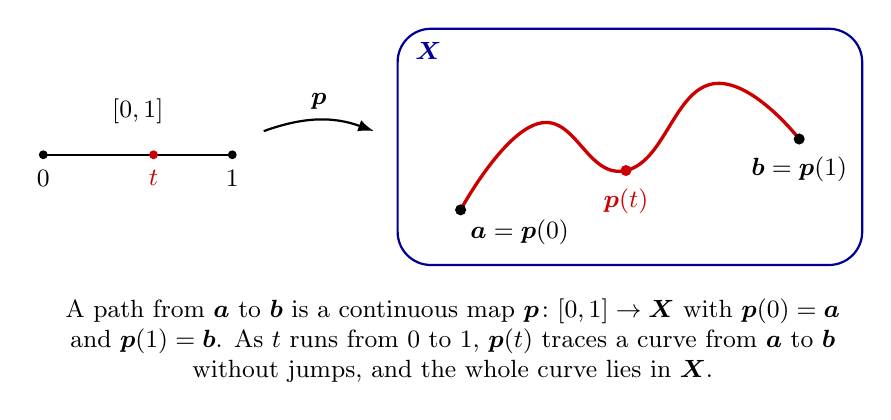
\begin{tikzpicture}[every node/.style={font=\small}, >={Latex[length=2mm]}]
	% the parameter interval [0,1]
	\draw[thick] (0,0) -- (2.4,0);
	\fill (0,0) circle (1.6pt) node[below=2pt] {$0$};
	\fill (2.4,0) circle (1.6pt) node[below=2pt] {$1$};
	\fill[red!80!black] (1.4,0) circle (1.6pt) node[below=2pt] {$t$};
	\node at (1.2,0.55) {$[0,1]$};
	% the map p
	\draw[->, thick] (2.8,0.3) to[bend left=20] node[midway, above] {$\boldsymbol{p}$} (4.2,0.3);
	% the space X and the curve p([0,1])
	\draw[blue!60!black, thick, rounded corners=12pt] (4.5,-1.4) rectangle (10.4,1.6);
	\node[blue!60!black, anchor=north west] at (4.6,1.55) {$\boldsymbol{X}$};
	\draw[very thick, red!80!black] plot[smooth, tension=0.8] coordinates {(5.3,-0.7) (6.3,0.4) (7.4,-0.2) (8.5,0.9) (9.6,0.2)};
	\fill (5.3,-0.7) circle (2pt) node[below right] {$\boldsymbol{a}=\boldsymbol{p}(0)$};
	\fill (9.6,0.2) circle (2pt) node[below=3pt] {$\boldsymbol{b}=\boldsymbol{p}(1)$};
	\fill[red!80!black] (7.4,-0.2) circle (2pt) node[below=3pt] {$\boldsymbol{p}(t)$};
	\node[anchor=north, align=flush center, text width=10cm] at (5.2,-1.7) {A path from $\boldsymbol{a}$ to $\boldsymbol{b}$ is a continuous map $\boldsymbol{p}\colon[0,1]\to\boldsymbol{X}$ with $\boldsymbol{p}(0)=\boldsymbol{a}$ and $\boldsymbol{p}(1)=\boldsymbol{b}$. As $t$ runs from $0$ to $1$, $\boldsymbol{p}(t)$ traces a curve from $\boldsymbol{a}$ to $\boldsymbol{b}$ without jumps, and the whole curve lies in $\boldsymbol{X}$.};
\end{tikzpicture}
\end{document}
